
\documentclass[a4paper,UKenglish,cleveref, autoref]{lipics-v2019}
%This is a template for producing LIPIcs articles. 
%See lipics-manual.pdf for further information.
%for A4 paper format use option "a4paper", for US-letter use option "letterpaper"
%for british hyphenation rules use option "UKenglish", for american hyphenation rules use option "USenglish"
%for section-numbered lemmas etc., use "numberwithinsect"
%for enabling cleveref support, use "cleveref"
%for enabling cleveref support, use "autoref"
\usepackage{xcolor}


%\graphicspath{{./graphics/}}%helpful if your graphic files are in another directory

\bibliographystyle{plainurl}% the mandatory bibstyle

\title{Formalizing double sided auctions in Coq} %TODO Please add

\titlerunning{}%optional, please use if title is longer than one line


\author{Abhishek Kr Singh}{Tata Institute of Fundamental Research, India} {abhishek.uor@gmail.com}
{}{}
\author{Suneel Sarswat}{Tata Institute of Fundamental Research, India} {suneel.sarswat@gmail.com}
{}{}

\authorrunning{Abhishek and Suneel}%TODO mandatory. First: Use abbreviated first/middle names. Second (only in severe cases): Use first author plus 'et al.'

\Copyright{Abhishek Kr. Singh and Suneel Sarswat}%TODO mandatory, please use full first names. LIPIcs license is "CC-BY";  http://creativecommons.org/licenses/by/3.0/

\ccsdesc[500]{Information systems~Online auctions}
\ccsdesc[500]{Software and its engineering~Formal software verification}
\ccsdesc[300]{Theory of computation~Algorithmic mechanism design}
\ccsdesc[300]{Theory of computation~Computational pricing and auctions}
\ccsdesc[100]{Theory of computation~Program verification}
\ccsdesc[100]{Theory of computation~Automated reasoning}


\keywords{Coq, formalization, auction, matching, financial markets }%TODO mandatory; please add comma-separated list of keywords

\category{}%optional, e.g. invited paper

\relatedversion{}%optional, e.g. full version hosted on arXiv, HAL, or other respository/website
%\relatedversion{A full version of the paper is available at \url{...}.}

\supplement{}%optional, e.g. related research data, source code, ... hosted on a repository like zenodo, figshare, GitHub, ...

%\funding{(Optional) general funding statement \dots}%optional, to capture a funding statement, which applies to all authors. Please enter author specific funding statements as fifth argument of the \author macro.

\acknowledgements{}%optional

%\nolinenumbers %uncomment to disable line numbering

%\hideLIPIcs  %uncomment to remove references to LIPIcs series (logo, DOI, ...), e.g. when preparing a pre-final version to be uploaded to arXiv or another public repository

%Editor-only macros:: begin (do not touch as author)%%%%%%%%%%%%%%%%%%%%%%%%%%%%%%%%%%
\EventEditors{}
\EventNoEds{2}
\EventLongTitle{}
\EventShortTitle{}
\EventAcronym{}
\EventYear{2019}
\EventDate{}
\EventLocation{}
\EventLogo{}
\SeriesVolume{}
\ArticleNo{}
%%%%%%%%%%%%%%%%%%%%%%%%%%%%%%%%%%%%%%%%%%%%%%%%%%%%%%

\begin{document}

\newcommand{\tw}{\texttt}

\maketitle

%TODO mandatory: add short abstract of the document
\begin{abstract}

In this paper we introduce a formal framework for analyzing double sided auction mechanisms in a theorem prover. In a double sided auction multiple buyers and sellers participate for trade. Any mechanism for double sided auctions to match buyers and sellers should satisfy certain properties. For example, fairness, percieved-fairness, individual rationality are some of the important properties. These are important properties and to verify them we need a formal setting. We formally define all these notions in a theorem prover. This provides us a  formal setting in which we prove some useful results on matching in a double sided auction. Finally, we use this framework to analyse properties of two important class of double sided auction mechanism. All the properties we discuss in this paper are completely formalized in the Coq proof assistant without adding any axiom to it.  
\end{abstract}

\section{Introduction}
\label{section1}

Trading is a principal component of all modern economy. Over the century more and more complex instruments (for example, index, future, options etc.) are being introduced to trade in the financial markets. With the arrival of computer assisted trading, the volume and liquidity in the markets has improved significantly. Today all big stock exchanges use computer algorithms (matching algorithms) to match buy requests (demands) with sell requests (supplies) of traders. Computer algorithms are also used by many traders to place orders  in the markets. This is known as algorithmic trading.  As a result of all this the markets has become complex and large. Hence, the analysis of markets is no more feasible without the help of computers. 

A potential trader (buyer or seller) places orders in the markets through a broker. These orders are matched by the stock exchange to execute trades. Most stock exchanges divide the trading activity into three main sessions known as pre-markets, continous markets and post markets. While in the pre-markets session an opening price of a product is discovered through double sided auction. In the continous markets session the incoming buyers and sellers are continously matched against each other on a priority basis. In the post-markets session clearing of the remaining orders is done and a closing price is discovered.

A double sided auction mechanism allows multiple buyers and sellers to trade simultaneously \cite{friedman}. In double sided auctions,  auctioneer (e.g. stock exchange) collects buy and sell requests over a period. Each potential trader places the orders with a \emph{limit price}: below which a seller will not sell and above which a buyer will not buy. The exchange at the end of this period matches these orders based on their limit prices. This entire process is completed using a matching algorithm for double sided auctions.  

Designing algorithms for double sided auctions is a well studied topic \cite{mcafee1992, WurmanWW98,NiuP13, ZhaoZKP10}.  A major emphasis of many of these algorithms is to maximize the number of matches or maximize the profit of the auctioneer. Note that an increase in the number of matches increases the liquidity in the markets. A matching algorithm can produce a matching with a uniform price or a matching with dynamic prices. While an algorithm which clears each matched bid-ask pair at a single price is referred as uniform price algorithm.  An algorithm which may clear each matched bid-ask pair at different prices is refered as  dynamic price algorithm. There are other important properties besides the number of macthes which are considered while evaluating the effectiveness of a matching algorithm. For example, fairness, uniform pricing, individual rationality are some of the relevant features used to compare these matching algorithms. However, it is known that no single algorithm can posses all of these properties \cite{WurmanWW98,mcafee1992}. 

In this paper, we describe a formal framework to analyze double sided auctions using a theorem prover.  For this work, we assume that each trader wishes to trade a single unit of the product and all the products are indistinguishable as well as indivisible. We have used the Coq proof assistant to formally  define the theory of double sided auctions.  Furthermore, we use this theory to validate various properties of matching algorithms. We formally prove some important properties of two algorithms; a uniform price algorithm and a dynamic price algorithm. 

\section{Modeling double sided auctions}
To formalize the notion of matching in a double sided auction we use  list data structure.  List is also used to define various processes that operate on  a matching. However, to express the properties of these processes we need some  relations on lists which are analogous to  relations on multisets. In this section we formally define these relations which are further used for stating some important results on matching in a double sided auction.

\subsection{Bid, Ask and limit price}
An auction is a  competitive event, where goods and services are sold to the highest bidders. In  any double sided auction multiple buyers and sellers place their orders to buy or sell a unit of underlying product. The  auctioneer then matches these buy-sell requests  based on their \emph{limit prices}. While the limit price for a buy order (i.e. \emph{bid}), is the price above which the buyer doesn't want to buy one quantity of the item. The limit price of a sell order (i.e. \emph{ask}), is the price below which the seller doesn't want to sell one quantity of the item.  In this work we assume that each bid is a buy request for one unit of item. Similarly each ask is a sell request for one unit of item. If a trader wishes to buy or sell multiple units, he can create multiple bids or asks with different \emph{ids}. 

We can express bid as well ask using  records containing two fields. 
\begin{verbatim}
  Record Bid: Type := Mk_bid { bp:> nat;    idb: nat }.
  Record Ask: Type := Mk_ask { sp:> nat;    ida: nat }.
\end{verbatim}
For a bid $b$, $(bp \; b)$  is the limit price and $(idb \; b)$ is its unique identity. Similarly for an ask $a$, $(sp \; a)$ is the limit price and $(ida \; a)$ is the unique identity of $a$. Note the use of coercion symbol \tw{ :>} in the first field of $Bid$. It declares $bp$ as an implicit function which is applied  to any term of type $Bid$ appearing in a context where a natural number is expected. Hence, now onward we can simply use $b$ instead of  ($bp \;b$) to express the limit price of $b$. Similarly we can use $a$ for the limit price of an ask $a$.


Since equality for both the fields of $Bid$ as well as $Ask$ is decidable (i.e. \tw{nat: eqType}), the equality on $Bid$ as well as $Ask$ can also be prooved decidable. This is achieved by declaring two canonical instances \tw{bid\_eqType} and \tw{ask\_eqType} which connect $Bid$ and $Ask$ to the \tw{eqType}.  

\subsection{Matching in Double Sided Auctions}
In a double sided auction (DSA), the auctioneer collects all the buy and sell requests for a fixed duration. All the buy requests can be assumed to be present in a list $B$. Similarly, all the sell requests can be assumed to be present in a list $A$. At the time of auction, the auctioneer matches bids in $B$ against asks in $A$. We say a bid-ask pair $(b, a)$ is \emph{matchable} if $b \ge a$ (i.e. $bp \; b \ge sp \; a$).  Furthermore, the auctioneer assigns a trade price to each matched bid-ask pair. This  process results in  a matching $M$, which consists of all the matched bid-ask pairs together with their trade prices. We define matching as a list whose entries are of type \tw{fill\_type}.
\begin{verbatim}
  Record fill_type: Type:=  Mk_fill {bid_of: Bid;  ask_of: Ask;  tp: nat} 
\end{verbatim}

In a matching $M$, a bid or an ask appears at most once. Note that there might be some bids in $B$ which are not matched to any ask in $M$. Similarly there might be some asks in $A$ which are not matched to any bid in $M$. The list of bids present in $M$ is denoted as $B_{M}$ and the list of asks present in $M$ is denoted as $A_M$. For example, Fig.~\ref{fig:matching} shows a matching $M$ between list of bids $B$ and list of asks $A$.  While the asks present in $A$ is shown using left brackets and corresponding limit prices. The bids present in $B$ is represented using right brackets and corresponding limit prices.  All the matched bid-ask pair in $M$ is then represented using  brackets of same colors. Note that the bid with limit price $37$ is not present in $B_M$ since it is not matched to any ask in $M$.  

\begin{figure}[h!]
\centering
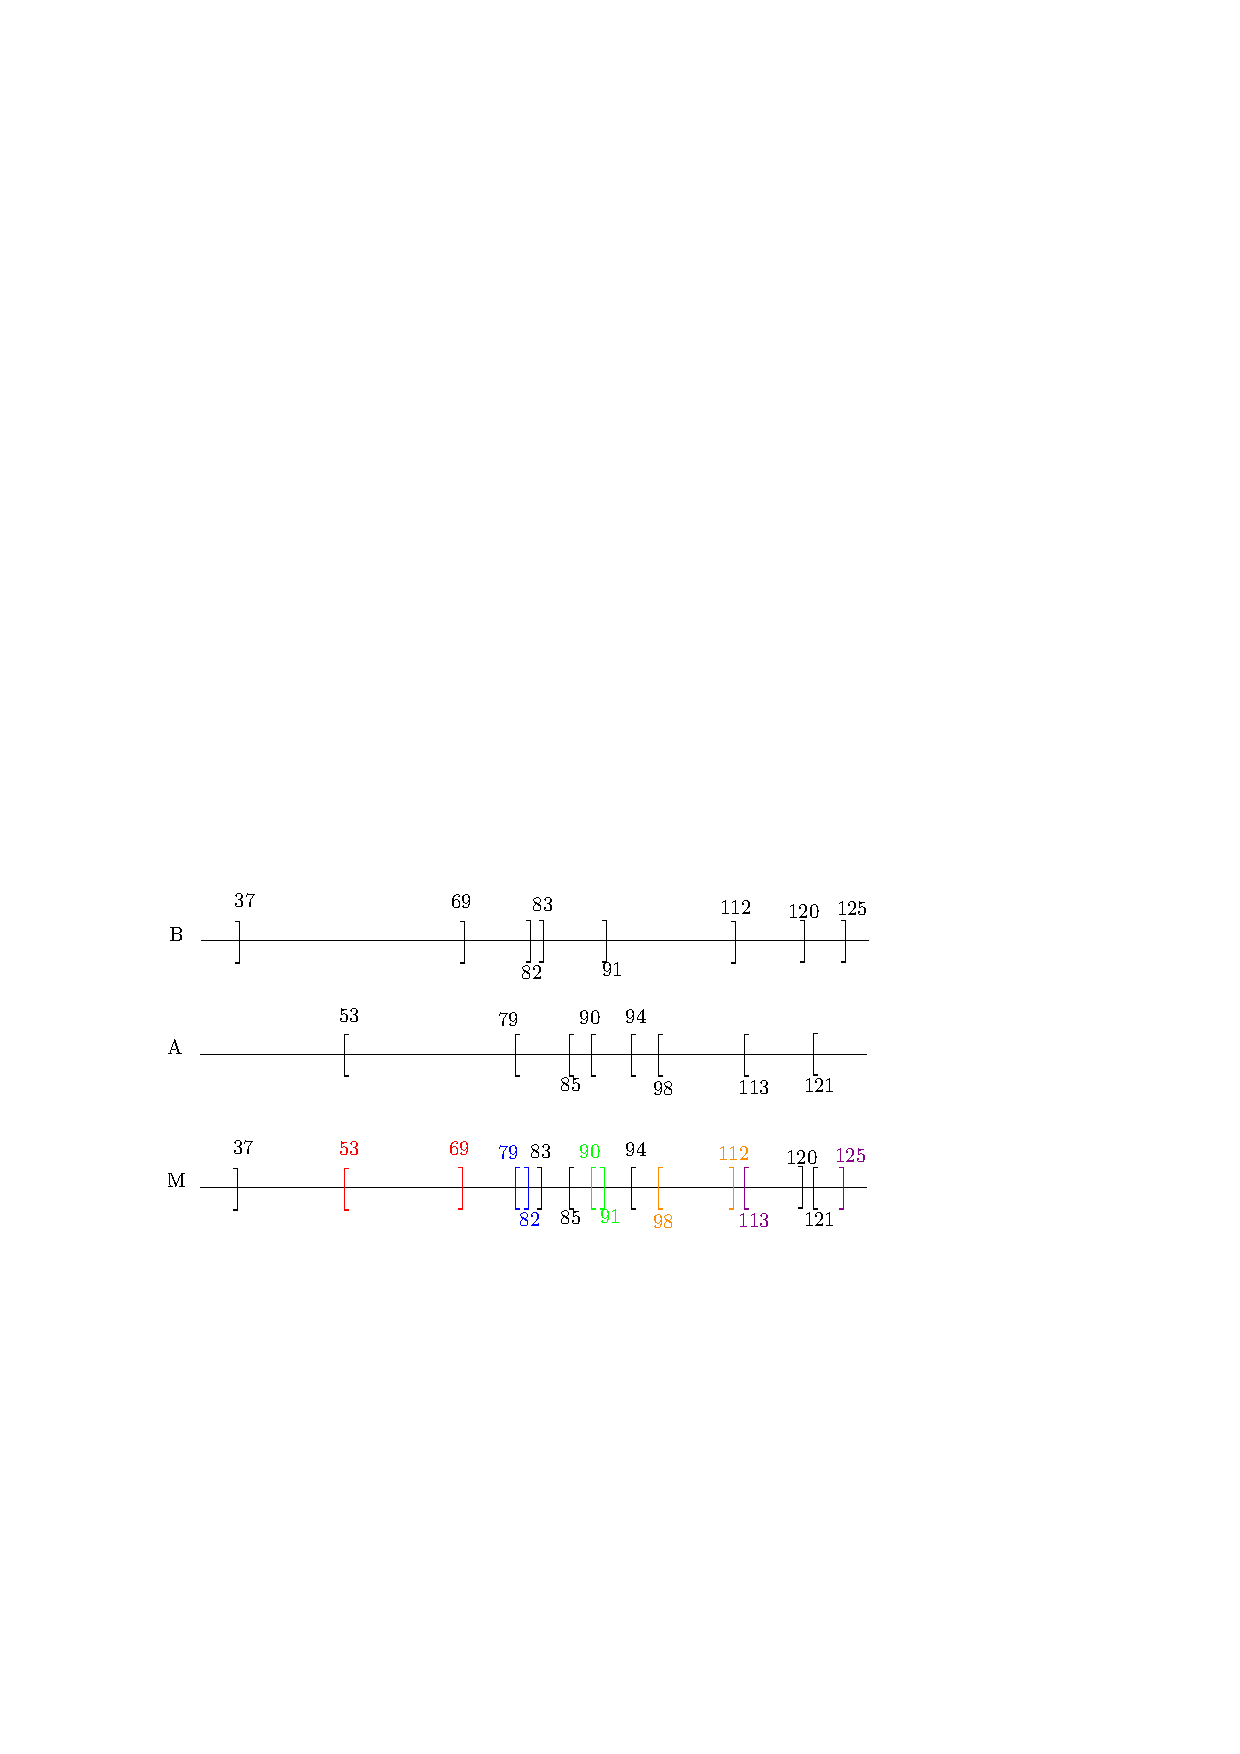
\includegraphics[width=.8\textwidth]{brack_matching.pdf}
\caption{ Bids in $B$ and asks in $A$ are represented using right and left brackets respectively. Every matched bid-ask pair in $M$ is shown using  brackets of same colors. Bids with limit prices $37$, $83$ and $120$ are not matched to any ask in the matching $M$.}
\label{fig:matching}
\end{figure}

More precisely, for a given list of bids $B$ and list of asks $A$, $M$ is a matching iff, (1) All the bid-ask pairs in $M$ are matchable, (2) $B_M$ is duplicate-free, (3) $A_M$ is duplicate-free, (4) $B_M \subseteq B$, and (5) $A_M \subseteq A$.

\begin{definition}
\tw{ \textcolor{gray}{matching\_in} B A M := All\_matchable M $\land$ NoDup $B_M$ $\land$ NoDup $A_M$ $\land$ $B_M \subseteq B$ $\land$ $A_M \subseteq A$.}
\end{definition}
While the term \emph{\tw{NoDup $B_M$}} in  above definition indicates that each bid is a request to trade one unit of item and the items are indivisible.  We use the expression $B_M \subseteq B$  to denote the term \tw{(Subset $B_M$ $B$)}.  It expresses the fact that each element in the list $B_M$ is also present in the list $B$.

\subsection{Lists, sublist and permutation}
While the predicates \tw{NoDup} and  \tw{Subset}  are sufficient to express the notion of a matching. We need more definitions to describe the properties of matching in double sided auctions.  In the following paragraphs we describe three binary relations on lists namely \tw{sublist}, \tw{included} and \tw{perm} which are then used for stating  important results on matching in a double sided auction. 

\begin{figure}[h!]
\centering
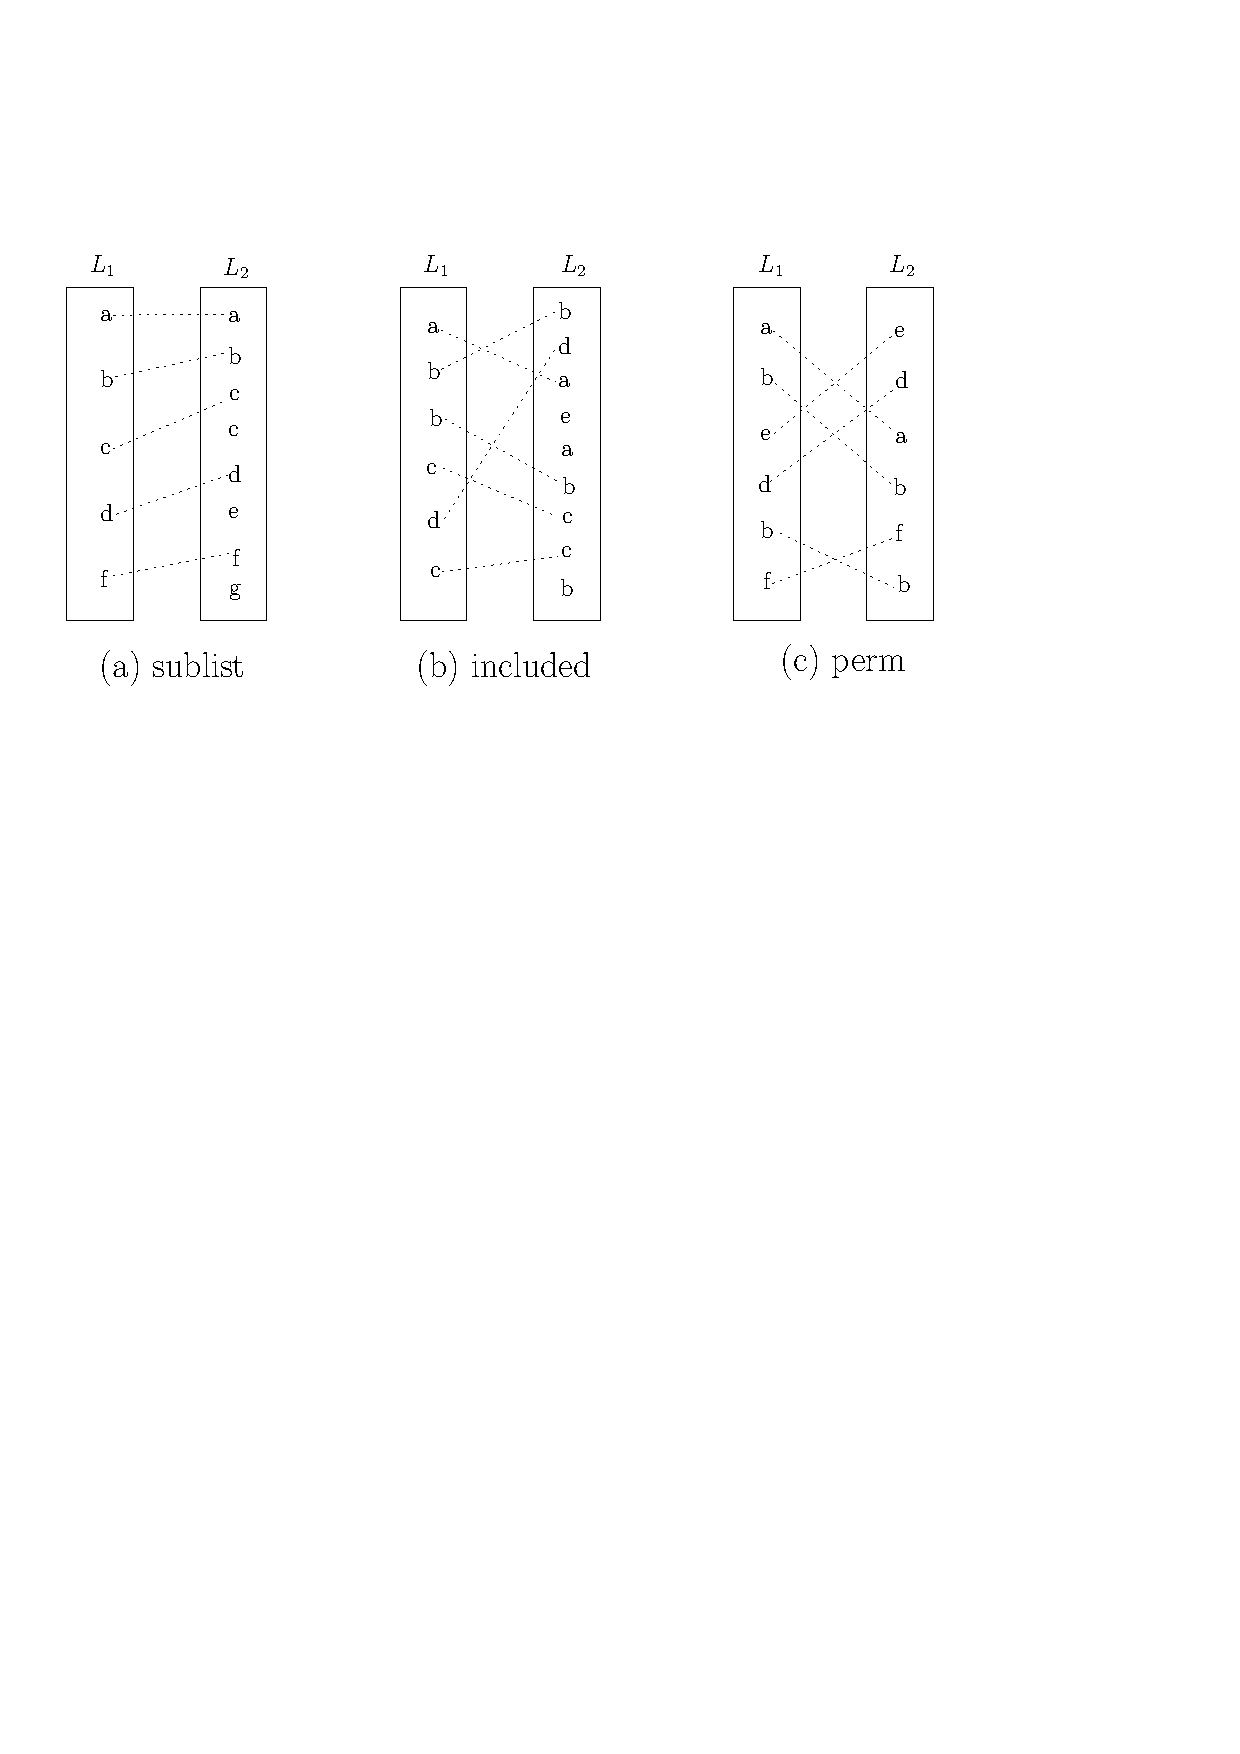
\includegraphics[width=.6\textwidth]{sub_inclu_perm.pdf}
\caption{The dotted lines between the entries of lists confirm the presence of these entries in both the lists. (a) If $L_1$ is \tw{sublist} of $L_2$ then no two dotted lines can intersect. (b) A list $L_1$ is \tw{included} in $L_2$ if every entry in $L_1$ is also present in $L_2$. (c) Two lists $L_1$ and $L_2$ are permutation of each other if each entry has same number of occurrences in both  $L_1$ and $L_2$. }
\label{fig:list}
\end{figure}

\subparagraph*{sublist $L_1$ $L_2$ :} The notion of \tw{sublist}  is analogous to the subsequence relation on sequences. For the given lists $L_1$ and $L_2$ the term  \tw{(sublist $L_1$ $L_2$)} evaluates to \tw{true}  if every entry of $L_1$ is also present in $L_2$ and they appear in the same succession.  For example, in Fig.~\ref{fig:list}(a) the list $L_1$ is a \tw{sublist} of $L_2$ since there is a line incident on each entry of $L_1$ and no two lines intersect each other. 

More precisely,  for any two lists $l$ and $s$ whose elements are of type \tw{T} we have following lemmas specifying the \tw{sublist} relation.

\begin{lemma} 
\tw{ \textcolor{gray}{sublist\_intro1} (a:T): sublist l s-> sublist l (a::s).}
\end{lemma}
\begin{lemma}\label{lem:sublistInd} 
\tw{ \textcolor{gray}{sublist\_elim3a} (a e:T): sublist (a::l)(e::s)-> sublist l s.}
\end{lemma}
\begin{lemma}\label{lem:subCount} 
\tw{ \textcolor{gray}{sublist\_elim4}: sublist l s -> ($\forall$ a, count a l $\leq$ count a s).}
\end{lemma}

The term (\emph{\tw{count a l}}) in Lemma~\ref{lem:subCount}  represents the number of occurrences of element $a$ in the list $l$. Note the recursive nature of \tw{sublist} as evident in Lemma~\ref{lem:sublistInd}. It  makes inductive reasoning easier for the statements which contain \tw{sublist} in the antecedent. However, this is  not true for the other relations (i.e. \tw{included} and \tw{perm}).

\subparagraph*{included $L_1$ $L_2$ :} A list $L_1$ is \tw{included} in  list $L_2$ if every entry of $L_1$ is also present in $L_2$. The notion of \tw{included}  is analogous to the subset relation on multisets. In Fig~\ref{fig:list}(b) the list $L_1$ is \tw{included} in $L_2$ since there is a line incident on each entry of $L_1$. More precisely, we have following lemmas specifying the \tw{included} relation.
\begin{lemma}
\tw{\textcolor{gray}{included\_intro}: ($\forall$ a, count a l $\leq$ count a s)-> included l s.}
\end{lemma}
\begin{lemma}
\tw{ \textcolor{gray}{included\_elim}: included l s -> ($\forall$ a, count a l $\leq$ count a s).}
\end{lemma}
\begin{lemma}
\tw{ \textcolor{gray}{included\_intro3}: sublist l s -> included l s. }
\end{lemma}

Note that if $l$ is \tw{sublsit} of $s$ then $l$ is also \tw{included} in $s$ but not the vice versa. However, if both the lists $l$ and $s$ are sorted based on some ordering on type \tw{T} then $l$ is \tw{sublist} of $s$ whenever $l$ is \tw{included} in $s$.
\begin{lemma}
\tw{ \textcolor{gray}{sorted\_included\_sublist}: Sorted l -> Sorted s -> included l s -> sublist l s.}
\end{lemma}

\subparagraph*{perm $L_1$ $L_2$ :} A list $L_1$  is permutation of list $L_2$  iff $L_1$  is included in $L_2$ and $L_2$ is included in $L_1$.  The notion of permutation for lists is simmilar to the equality in multisets. In Fig~\ref{fig:list}(c) the list $L_1$  is perm of list $L_2$. We have following lemmas specifying the essential properties of the \tw{perm} relation.

\begin{lemma}
\tw{ \textcolor{gray}{ perm\_intro}: ($\forall$ a, count a l = count a s) -> perm l s.}
\end{lemma}
\begin{lemma}
\tw{ \textcolor{gray}{perm\_elim}: perm l s -> ($\forall$ a, count a l = count a s).}
\end{lemma}
\begin{lemma}\label{lem:permSort}
\tw{ \textcolor{gray}{perm\_sort}(e: T-> T-> bool): perm l s -> perm  l (sort e s).}
\end{lemma}

The term (\emph{\tw{sort s}}) in Lemma~\ref{lem:permSort} represents the list $s$ sorted using an ordering relation \tw{e}. The definition of matching as a list is neccessary for describing processes that operate on it. However, while describing various properties of a matching we can always consider it as a collection. For example, consider the following lemma which states that the property of  being a matching is invariant over permutation. 
\begin{lemma}
\tw{\textcolor{gray}{match\_inv}: perm M  M' -> perm B B' -> perm A A' -> matching\_in B A M -> matching\_in B' A' M'. }
\end{lemma}
-----> Motivate and explain projection functions and corresponding lemmas. 
% Write about the projection functions  why needed and its  lemma and it's essence. 

\begin{lemma}
\tw{ \textcolor{gray}{ } }
\end{lemma}







\section{Analysis of Double sided auctions}
Usually in a double sided auctions mechanism, the profit of an auctioneer is the difference between the limit prices of matched bid-ask pair. In this work we do not consider analysis of profit for the aiuctioneer. Therefore the buyer of matched bid-ask pair pays the same amout which seller recieves. This price for a matched  bid-ask pair is called the trade price for that pair. Since the limit price for a buyer is the price above which she doesn't want to buy, the trade price for this buyer is expected to be below its limit price. Similarly the limit price for a seller is the price below which he doesn't want to sell, hence the trade price for this seller is expected to be be below its limit price. Therefore it is desired that in any matching the trade price of a bid-ask pair lies between their limit prices. A matching which has this property is called an \emph{indivial rational (IR)} matching. Note that any matching can be converted to an IR matching without altering it's bid-ask pair (See Fig~\ref{fig:IR}).

\begin{figure}[h!]
\centering
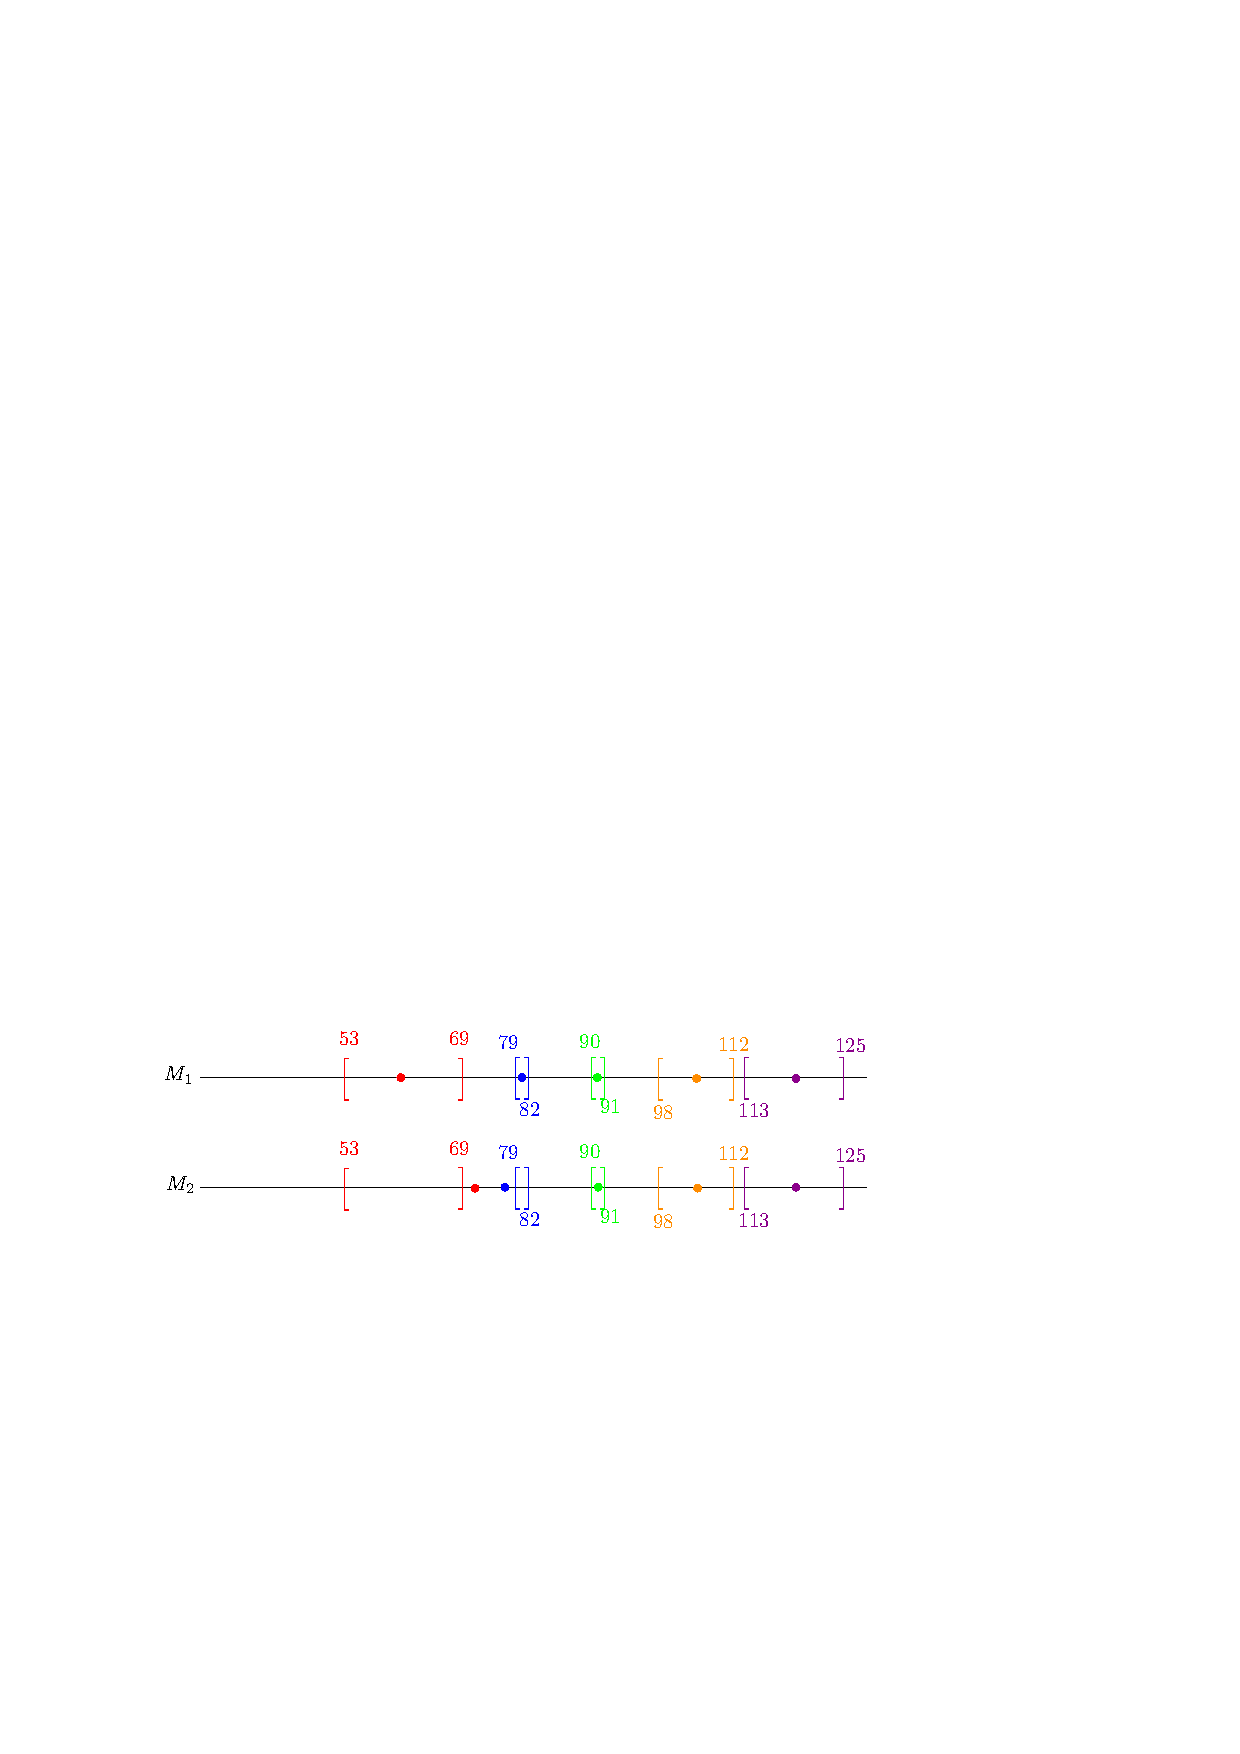
\includegraphics[width=.8\textwidth]{brack_IR.pdf}
\caption{ The colored dots represent the trade prices at which the corresponding matched bid-ask pairs are traded. While the matching $M_2$ is not IR since some dots lie outside the corresponding matched bid ask-pair. The matching $M_1$ is IR because trade prices for every matched bid-ask pair  lie inside the interval. Note that the matching $M_1$ and $M_2$ contains exactly same bid-ask pairs.}
\label{fig:IR}
\end{figure}

The number of matched bid-ask pairs produced by any matching algorithm is crucial in the design of a double sided auction mechanism. Increasing the number of matched bid-ask pairs increases the liquidity in market. Therefor, producing a maximum matching is an important aspect of double sided auction mechanism design. For a given list of bids $B$ and list of asks $A$ we say a matching $M$ is a maximum matching if no other matching $M'$ on the same $B$ and $A$ contains more number of matched bid-ask pairs than $M$. 

\begin{definition}
\tw{ \textcolor{gray}{Is\_MM} M B A := (matching\_in B A M) $\land$ 
($\forall$ M', matching\_in B A M' $\rightarrow$ |M'| $\leq$ |M|)}.
\end{definition}

In certain situations, to produce a maximum matching, different bid-ask pair must be assigned different trade prices. However, different prices for the same product in the same market simultaneausly leads to dissatisfaction amongst some of the traders. A machanism which clears all the matched bid-ask pairs at same trade price is called a \emph{uniform matching}. It is also known as percived-fairness (cite). In many situation it is not possible to produce an IR matching which is maximum and uniform at the same time. For example in Fig ~\ref{fig:mmum} a maximum matching of size two is possible but any uniform matching of size more than one in not possible. 


\begin{figure}[h!]
\centering
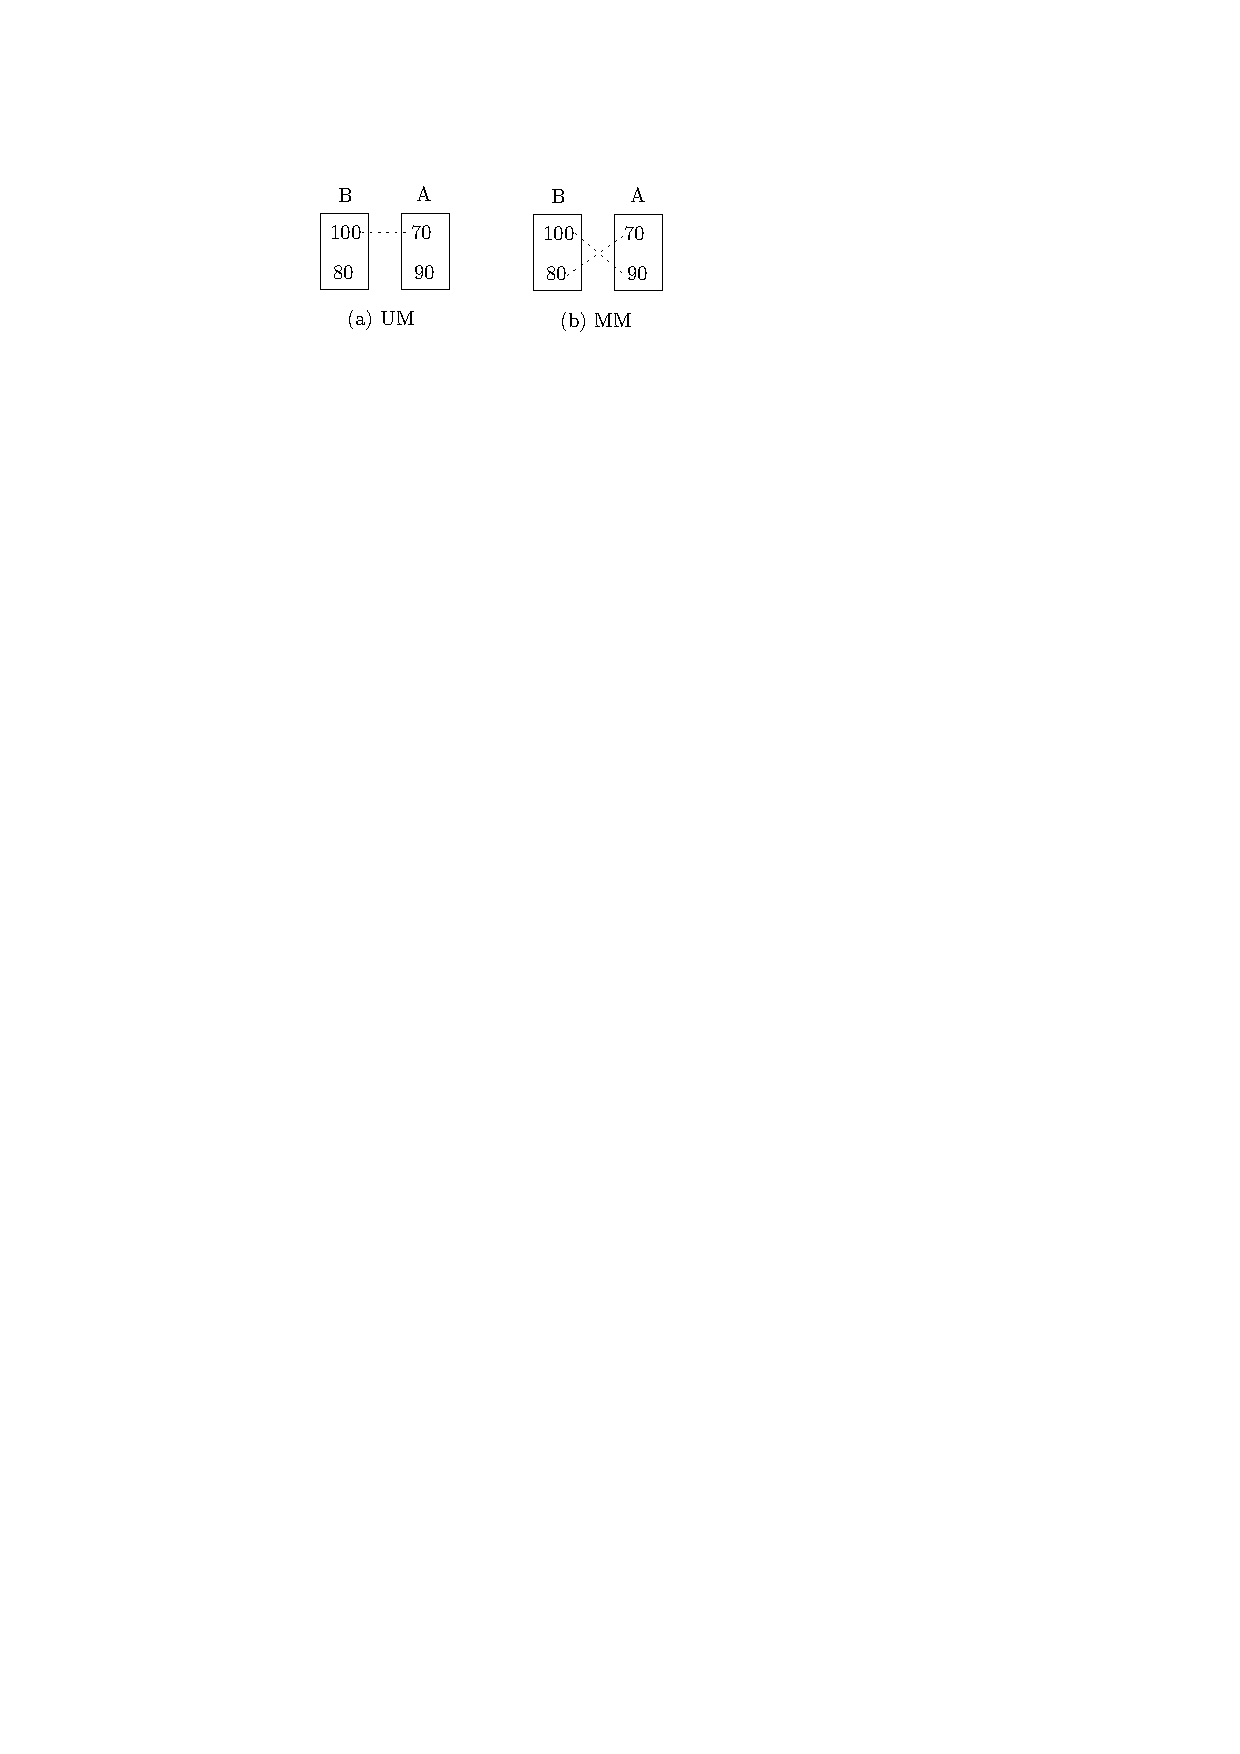
\includegraphics[width=.5\textwidth]{mm_um.pdf}
\caption{In this figure two bids with limit prices 100 and 80 respectively are matched against two asks of limit price 70 and 90. There is only one matching $M_2$ of size two possible and it is not uniform.}
\label{fig:mmum}
\end{figure}


\subsection{Fairness}  

A bid with higher limit price is more competitive campared to bids with lower limit prices. Similaly an ask with lower limit price is more competitive campared to asks with higher limit prices. In a campetitive market, like double sided auction, it is neccesory to priortise more competitive traders for matching. A matching which priortise competitive traders is a fair matching. Consider the following predicates \tw{fair\_on\_bids} and  \tw{fair\_on\_asks} which can be used to describe a fair matching. 

\begin{definition}
\tw{ \textcolor{gray}{fair\_on\_bids} M B:=
$\forall$ b b', In b B $\land$ In b' B -> b $>$ b' -> In b' $B_M$ -> In b $B_M$.}
 \end{definition}
\begin{definition}
\tw{ \textcolor{gray}{fair\_on\_asks} M A:=
$\forall$ s s', In s A $\land$ In s' A -> s $<$ s' -> In s' $A_M$ -> In s $A_M$. }
\end{definition}
\begin{definition}
\tw{ \textcolor{gray}{Is\_fair} M B A:=
fair\_on\_asks M A $\land$ fair\_on\_bids M B.}
\end{definition}

Here, the predicate \tw{fair\_on\_bids M B}  denotes that the matching $M$  is fair for the list of buyers $B$. Similarly,  the predecate \tw{fair\_on\_asks M A} assures that the matching $M$  is fair for the list of sellers $A$.  A matching which is fair on both the traders (i.e. $B$ and $A$) is expessed using the predecate \tw{Is\_fair M B A}.

Unlike the uniform matching a fair matching can always be achieved without compromising the the size the matching. We can accopmlish this by converting any matching into a fair matching without changing its size. For example consider the following function \tw{make\_FOB}.

\begin{verbatim}
	  Fixpoint Make_FOB (M:list fill_type) (B: list Bid):=
	    match (M,B) with 
	    |(nil,_) => nil
	    |(m::M',nil) => nil
	    |(m::M',b::B') => (Mk_fill b (ask_of m) (tp m))::(Make_FOB M' B')
	  end.
\end{verbatim}


The function \tw{make\_FOB} produces \tw{fair\_on\_bids} matching from a given matching M and a list of bids B, both sorted in decresing order bid prices (See Fig~\ref{fig:fair}). The function \tw{make\_FOB} is a recursive function and it replaces the largest bid in M with the largest bid in B. Since at any moment the largest bid in B is bigger than the largest bid in M, the new bid-ask pair is still matchable. Note that \tw{make\_FOB} doesn't change any of the ask in M and due to recursive nature of \tw{make\_FOB} on B, a bid is not repeated in the process of replacement.  This ensure that the new $B_M$ is duplicate-free. Once a matching is modified to a fair matching on bids, we use similar function \tw{make\_FOA} on this matching to produce a fair on ask matching. Hence the final result is a fair matching. 

\begin{figure}[h!]
\centering
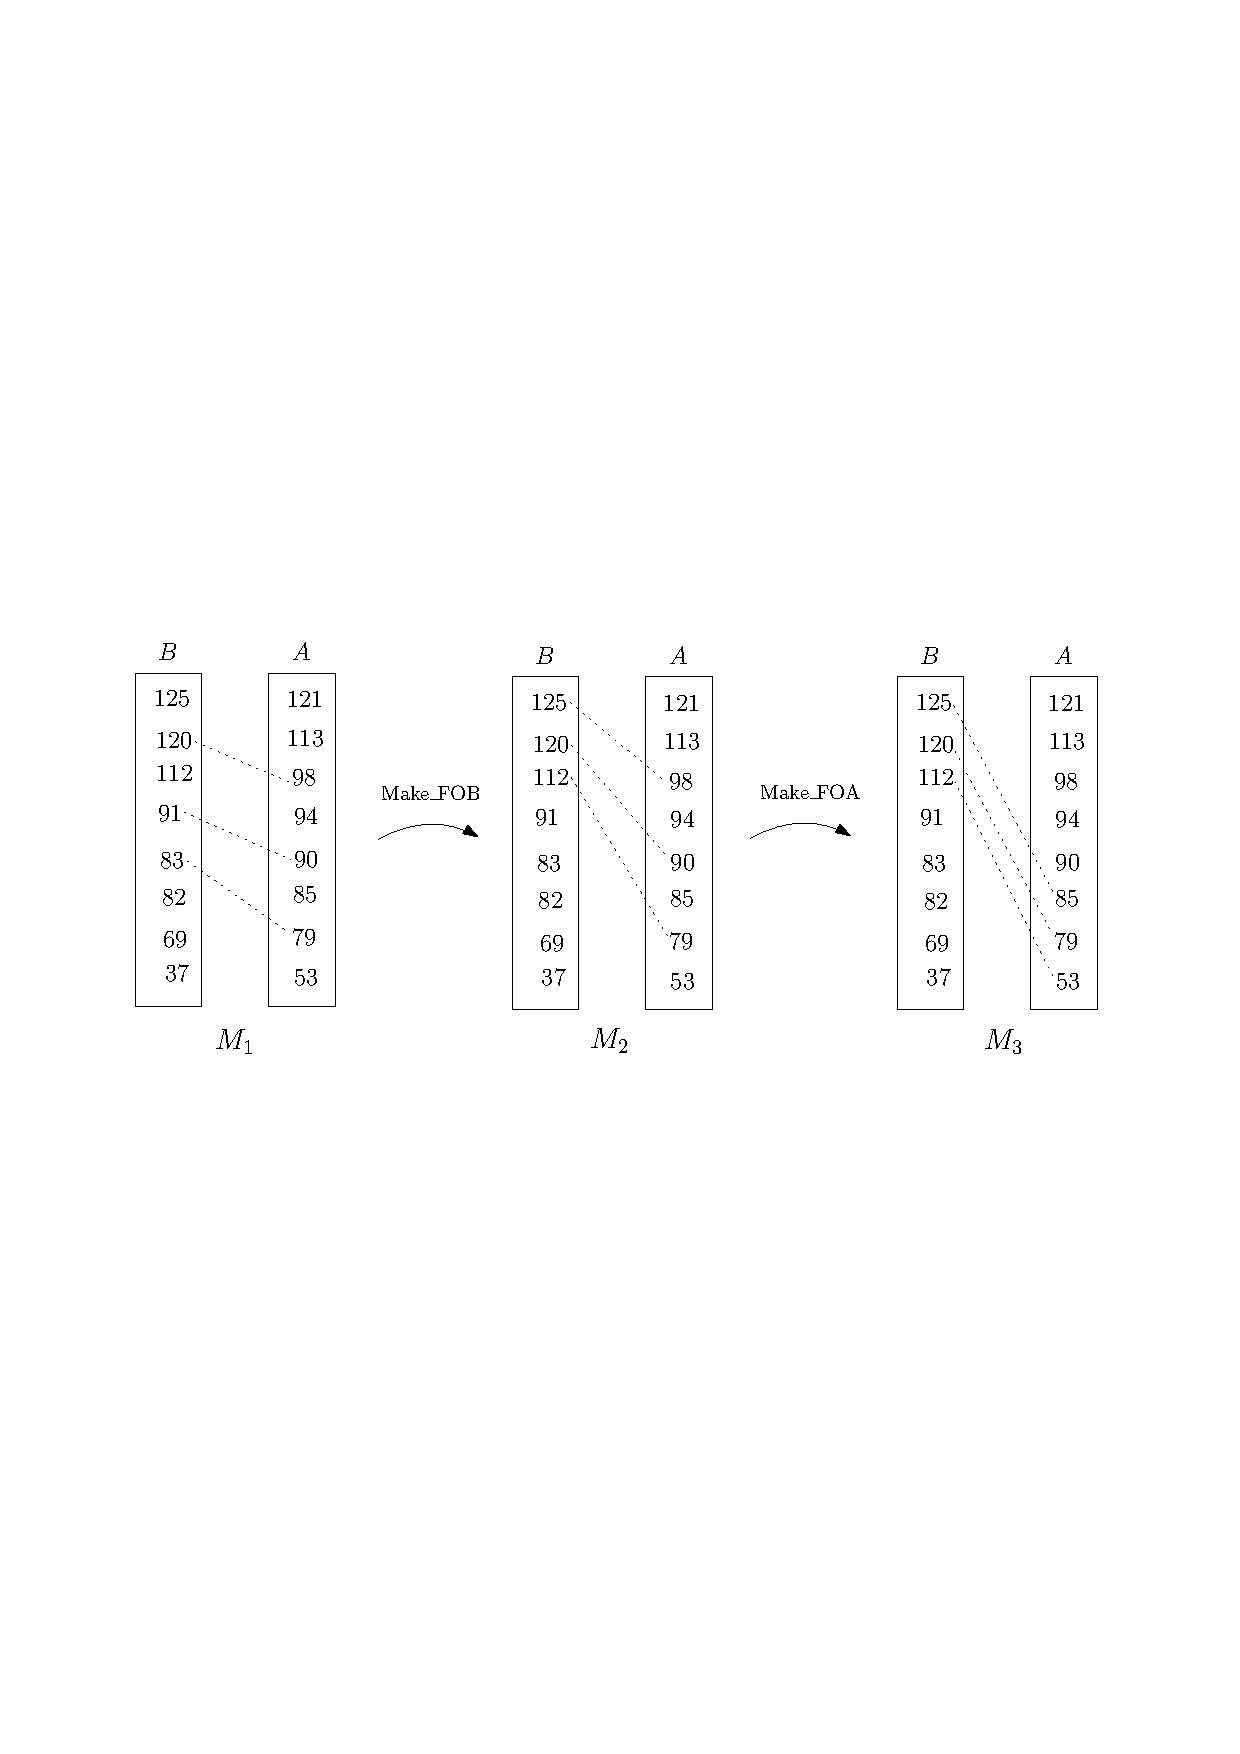
\includegraphics[width=.8\textwidth]{make_fair.pdf}
\caption{The dotted lines in this figure respresent  matched bid-ask pairs in  matching $M_1$, $M_2$ and $M_3$. In the first step function \tw{make\_FOB} operates on $M_1$ recursively. At each step it picks the top bid-ask pair, say $(b,a)$ in $M_1$ and replaces the bid  $b$ with most competitive bid available in $B$. The result of this process is a \tw{fair\_on\_bids} matching $M_2$. In a similar way the function \tw{make\_FOA} changes $M_2$ intro a fair on ask matching $M_3$.  }
\label{fig:fair}
\end{figure}

For the function \tw{make\_FOB} we have following lemma prooving it fair on bids. 
\begin{lemma}
\tw{ \textcolor{gray}{mfob\_fair\_on\_bid} M B A:
  (Sorted M) -> (Sorted B) -> sublist (bid_prices (bids_of M)) (bid_prices B) ->
  fair_on_bids (Make_FOB M B) B.  }
\end{lemma}

\begin{verbatim}
Lemma mfob_fair_on_bid (M: list fill_type) (B:list Bid) (A:list Ask):
  (Sorted m_dbp M) -> (Sorted by_dbp B) -> sublist (bid_prices (bids_of M)) (bid_prices B) ->
  fair_on_bids (Make_FOB M B) B. 
\end{verbatim}
The proof of above fact is using induction on the size of matching. Note we have not kept matching in the antecedent. For example we get stuck in induction if we try to prove the following claim directly using induction.

--> Insert Claim.
Try to signify the role of sublist and how it helps. 

---> Explain the final result on fairness
\begin{verbatim}
Theorem exists_fair_matching (M: list fill_type) (B: list Bid) (A:list Ask) (NDB: NoDup B) (NDA: NoDup A):
  matching_in B A M-> (exists M':list fill_type, matching_in B A M' /\ Is_fair M' B A /\ |M|= |M'|).
\end{verbatim}


\subsection{Maximum Matching}

The liquidity in any market is a meausre of how quickly one can trade in the market without much cost. A highly liquid market boosts the investor's confidence in the market. One way to increase the liquidity in a double sided auction is to maximize the number of matched bid-ask pair. In the previous section we have seen that any matching can be changed to a fair matching without altering its size. Therefore, we can have a maximum matching without compromising on the fairness of the matching. In this section we describe a matching which fair as well as maximum. For a given bid B and ask A, a maximum and fair matching can achieved in two steps. In first we have function \tw{produce\_MM} which produce a matching which is maximum and fair on bids. In the next step we apply \tw{make\_FOA} to this maximum matching to produce a fair on ask matching (See Fig~\ref{fig:mm}).

\begin{figure}[h!]
\centering
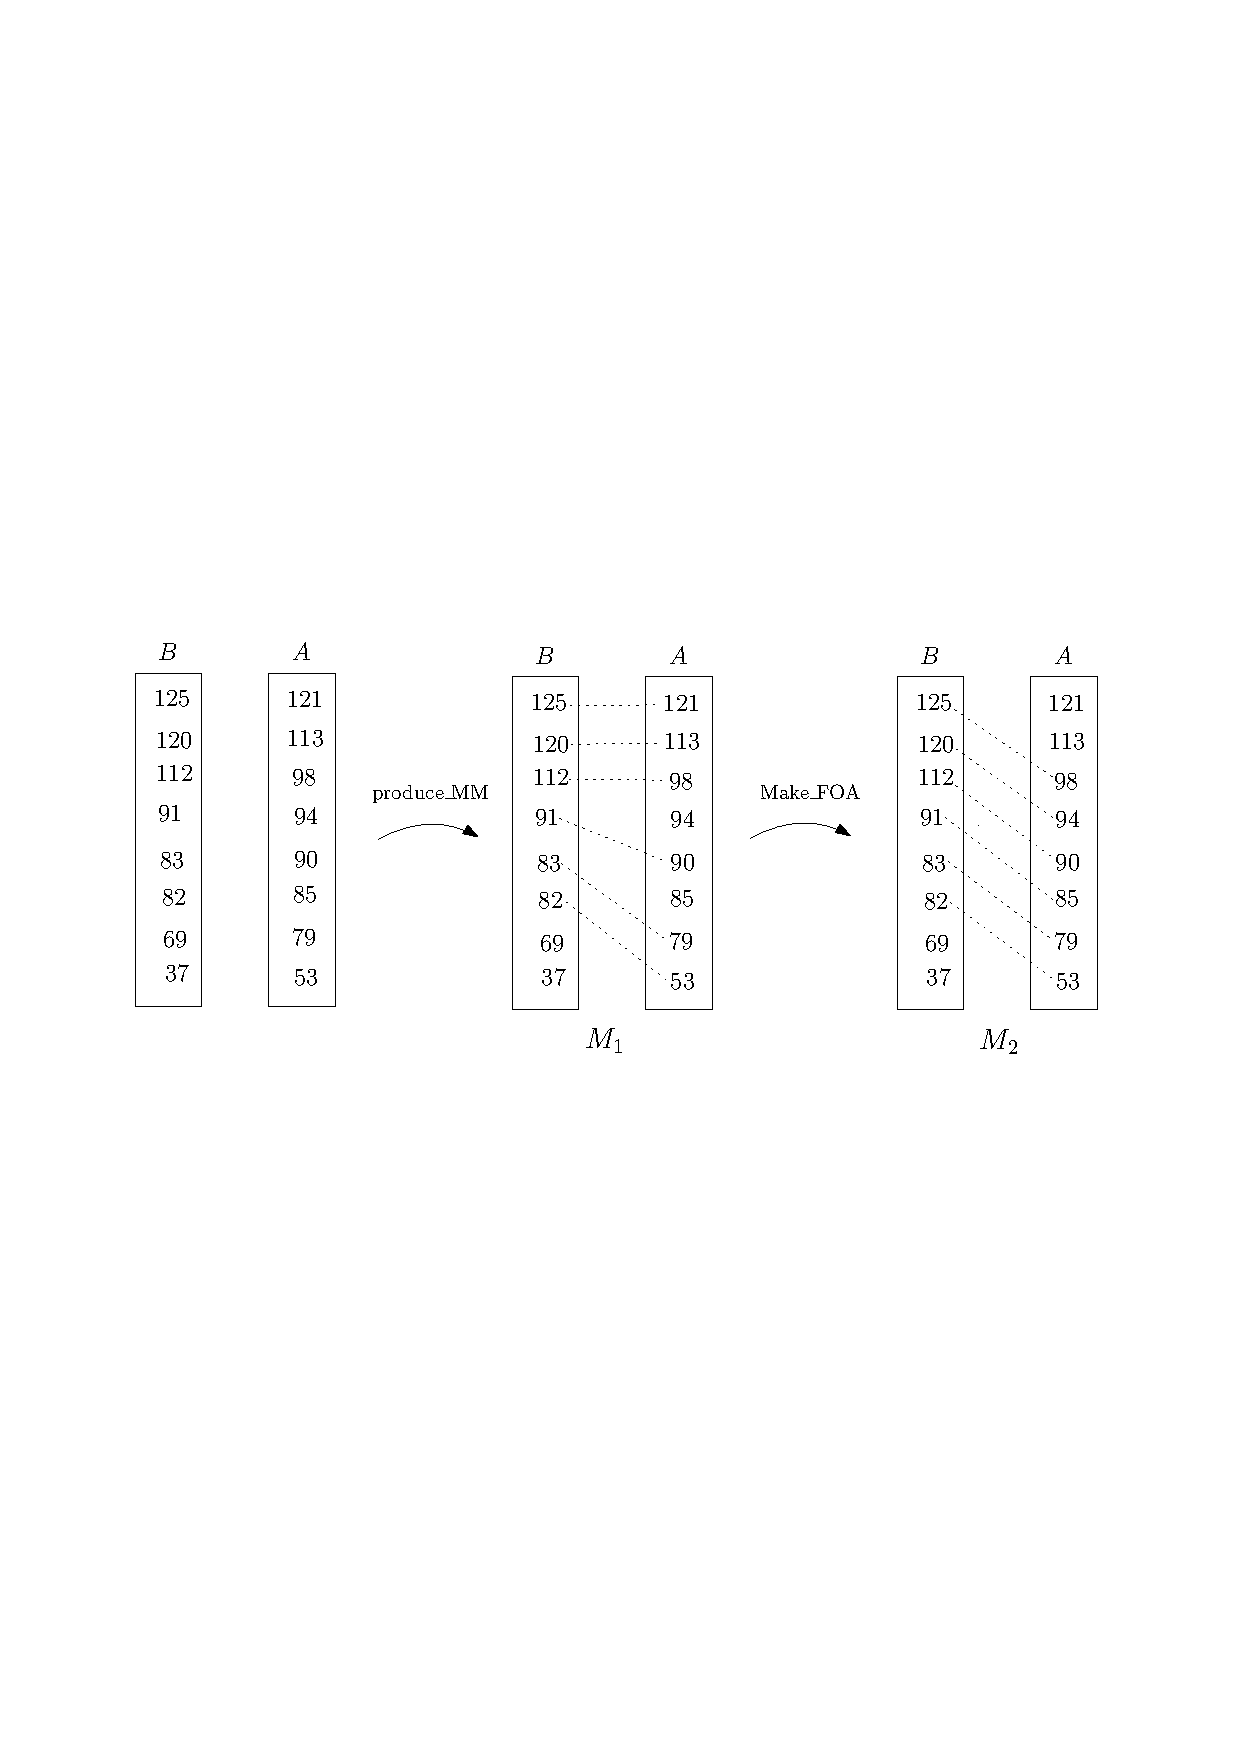
\includegraphics[width=.8\textwidth]{MM.pdf}
\caption{In the first step, the function \tw{produce\_MM} operates reccursively on the list of bids B and list of asks A. At each step the function \tw{produce\_MM} selects the most competitive available bid and then pairs it with the largest mathchable ask. Note that the output of this function is fair on bid since it doesn't leave any bid from top. In the second step, the function \tw{make\_FOA} converts the $M_1$ into fair matching $M_2$. }
\label{fig:mm}
\end{figure}

\begin{verbatim}
Fixpoint produce_MM (B:list Bid) (A: list Ask): (list fill_type) :=
  match (B, A) with
  |(nil, _) => nil
  |(b::B', nil) => nil              
  |(b::B', a::A') => match (Nat.leb (sp a) (bp b)) with
                    |true => ({|bid_of:= b ; ask_of:= a ; tp:=(bp b) |})::(produce_MM B' A')
                    |false => produce_MM B A'
                    end
  end. 
\end{verbatim}
--> edit the above definition.

The function \tw{produce\_MM} produces a maximum matching from a given lists of bids B and a list of asks A, both sorted in decresing order by limit prices (See Fig~\ref{fig:MM}). At each iteration it generates a matchable bid-ask pair. Due to the recursive nature of  function  \tw{produce\_MM} on both B and A, it never pair any bid with more than two asks. This ensures that the list of bids in matching $B_M$ is duplicate-free. Note that the function \tw{produce\_MM} tries to match a bid until it finds a matchable ask before pairing the next bid. The function terminates when either all the bids are matched or it encounters a bid for which no matchable ask is available. Therefore, it produces a matching which is fair on bid.

\begin{verbatim}
 Lemma produce_MM_fob (B: list Bid)(A: list Ask):
   Sorted by_dbp B -> Sorted by_dsp A -> fair_on_bids (produce_MM B A) B.
\end{verbatim}

Talk about the maximality proof. 
\begin{verbatim}
Lemma produce_MM_is_MM (B: list Bid)(A: list Ask)(no_dup_B: NoDup B)(no_dup_A: NoDup A):
   Sorted by_dbp B -> Sorted by_dsp A-> Is_MM (produce_MM B A) B A.
\end{verbatim}
---> Insert the proof diagram 
---> Proof Idea. 

---> Final lemmas stating that there exists a maximal and fair matching.
\begin{verbatim}
Theorem exists_fair_maximum (B: list Bid)(A: list Ask): exists M, (Is_fair M B A /\ Is_MM M B A).
\end{verbatim}


\section{Matching in financial markets} 
An exchange is an organized financial market. There are various types of exchanges for example stock exchange, commodity exchange, foreign exchange etc. The job of the exchange is to facilitate trading between buyers and sellers for the products which are registered in the exchange. Many exchanges operates during a fix duartion in the day. Some exchanges devides the trading activities into multiple sessions for various reseaons. Many stock exchanges hold trading into two main session; pre-market or auction session and continous market or regular trading session. During the pre-market session an exchange collects all the bids and asks for fix duration and then apply double sided auction mechanism to these orders. At the end of the pre-market session an opening price for the product is deiscovered. During the regular sessions a bid (ask) is matched against the existing asks (bids) immedietly. If the bid (ask) is not matchable it is placed in the priority queue based on their limit price. 

The pre-market session reduces uncertenity and volatilty for the regular sessions of trading. To avoid failure on behalf of the traders the exchange must match all the bids or asks withing their limit price. So any matching produced during this session must be indivdual rational. Furthermore, the exchange must be fair towards all the traders. So the matching produced during this session be should be fair matching. One of the most important aspects of the pre-market session is to descover the price of underlying product based on the total demand and supply. This means there must be a unique price at which all the matched bid-ask pairs shuold be traded. So any matching produced during this session should produce a uniform matching. 

Most exchanges matches the bids and asks during the pre-market session at eqilibrium price.  An equlibrium price is the price at which maximum number of bids can be matched with maximum number of asks. We describe an algorithm which produces an equilibrium price. The algorithm \tw{UM} produces a individual rational matching which is fair and maximum amongst uniform matchings.

\begin{verbatim}
Fixpoint produce_UM (B:list Bid) (A:list Ask)  :=
  match (B,A) with
  |(nil, _) => nil
  |(_,nil)=> nil
  |(b::B',a::A') => match Nat.leb (sp a) (bp b) with
                 |false =>nil
                  |true  => ({|bid_of:= b ; ask_of:= a ; tp:=(bp b) |})::produce_UM B' A'
  end
end.

Definition uniform_price (B: list Bid) (A: list Ask):=
  (bp (bid_of (last (UM_matching B A) ((b0,a0),0)))).

Definition UM (B:list Bid) (A:list Ask) : (list fill_type) :=
  replace_column (UM_matching B A) (uniform_price B A).

\end{verbatim}


The function \tw{produce\_UM} produces bid-ask pairs, \tw{uniform\_price} discover the uniform price and finally \tw{UM} produces a uniform matching. The function \tw{produce\_UM} is a recursive function which matches the largest bid with the smallest ask at each iteration (See Fig~\ref{fig:UM.pdf}). The function terminates when a bid is not matchable with an ask. Observe that in any individual rational and uniform matching the number of bids above to the trade price is same as the number of asks below to the trade price. Let $M$ be any arbitrary IR and uniform matching of size $k$ with trade price $t$. Then there are atleast $k$ bids above $t$ and $k$ asks below $t$. So natuaraaly there are at least $k$ largest bids matchable with $k$ smallest asks. Since UM algorithm pair largest bid with the smallest bid in each iteration then UM must pair at least $k$ bids with $k$ asks. Hence UM produce a matching which of size at least $k$. Therefore UM produces an IR and fair matching which maximum amongst uniform matchings. 

\begin{theorem}
\tw{
\textcolor{gray}{UM\_is\_maximal\_Uniform} (B: list Bid) (A:list Ask): $\forall$ M: list fill\_type, Is\_uniform M -> |M| $\leq$ | (UM B A ) |
}
\end{theorem}


\section{Conclusion}
There has been many attempt in past to design various algorithms for double sided auctions \cite{Deshmukh:2002:TCD}. Fairness, individual rationality and uniformity are some of the critical properties on which effectiveness of these algorithms are evaluated. Theorem provers can be a  useful  tool in the analysis of these properties \cite{oai:HAL:hal-01673716v1, standLib}. There is an attempt to formalize the financial markets in theorem prover \cite{PassmoreI17}. Our work is the first attempt in formalizing double sided auction in a theorem prover. Formalizing the double sided auction in a theorem proover increases the reliability of the mechanism. Our work in future can be extended for any number of units.  


%% Bibliography
\bibliography{auction}

\end{document}
